\documentclass[preview,border={20pt 20pt 20pt 20pt}]{standalone}
\usepackage{tikz,pgfplots}
\usepackage{fancyvrb}
\usepackage{xcolor}\begin{document}
\begin{figure}[h]
\centering
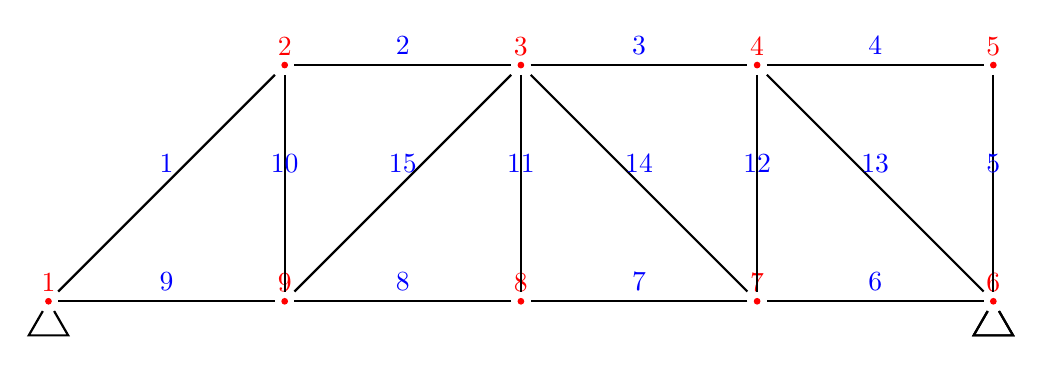
\begin{tikzpicture}
\draw node(1)[mark size=1pt, color = red] at (0,0) {\pgfuseplotmark{*}};
\draw node[above, red] at (0,0) {1};
\draw node(2)[mark size=1pt, color = red] at (3,3) {\pgfuseplotmark{*}};
\draw node[above, red] at (3,3) {2};
\draw node(3)[mark size=1pt, color = red] at (6,3) {\pgfuseplotmark{*}};
\draw node[above, red] at (6,3) {3};
\draw node(4)[mark size=1pt, color = red] at (9,3) {\pgfuseplotmark{*}};
\draw node[above, red] at (9,3) {4};
\draw node(5)[mark size=1pt, color = red] at (12,3) {\pgfuseplotmark{*}};
\draw node[above, red] at (12,3) {5};
\draw node(6)[mark size=1pt, color = red] at (12,0) {\pgfuseplotmark{*}};
\draw node[above, red] at (12,0) {6};
\draw node(7)[mark size=1pt, color = red] at (9,0) {\pgfuseplotmark{*}};
\draw node[above, red] at (9,0) {7};
\draw node(8)[mark size=1pt, color = red] at (6,0) {\pgfuseplotmark{*}};
\draw node[above, red] at (6,0) {8};
\draw node(9)[mark size=1pt, color = red] at (3,0) {\pgfuseplotmark{*}};
\draw node[above, red] at (3,0) {9};
\draw[thick] (1) -- node[above, blue]{1} (2);
\draw[thick] (2) -- node[above, blue]{2} (3);
\draw[thick] (3) -- node[above, blue]{3} (4);
\draw[thick] (4) -- node[above, blue]{4} (5);
\draw[thick] (5) -- node[above, blue]{5} (6);
\draw[thick] (6) -- node[above, blue]{6} (7);
\draw[thick] (7) -- node[above, blue]{7} (8);
\draw[thick] (8) -- node[above, blue]{8} (9);
\draw[thick] (9) -- node[above, blue]{9} (1);
\draw[thick] (9) -- node[above, blue]{10} (2);
\draw[thick] (3) -- node[above, blue]{11} (8);
\draw[thick] (4) -- node[above, blue]{12} (7);
\draw[thick] (4) -- node[above, blue]{13} (6);
\draw[thick] (3) -- node[above, blue]{14} (7);
\draw[thick] (3) -- node[above, blue]{15} (9);
\draw[thick] (1) -- ++(-0.25,-0.4330127019) -- ++(0.5,0) -- (1);
\draw[thick] (6) -- ++(-0.25,-0.4330127019) -- ++(0.5,0) -- (6);
\draw[thick] (6) -- ++(-0.25,-0.4330127019) -- ++(0.5,0) -- (6);
\end{tikzpicture}
\end{figure}
\begin{Verbatim}[commandchars=\\\{\}]
The force in member \textcolor{blue}{1} is -47.03 kN
The force in member \textcolor{blue}{2} is -33.26 kN
The force in member \textcolor{blue}{3} is -29.42 kN
The force in member \textcolor{blue}{4} is -0.00 kN
The force in member \textcolor{blue}{5} is  0.00 kN
The force in member \textcolor{blue}{6} is 47.10 kN
The force in member \textcolor{blue}{7} is 56.52 kN
The force in member \textcolor{blue}{8} is 56.52 kN
The force in member \textcolor{blue}{9} is 33.26 kN
The force in member \textcolor{blue}{10} is 33.26 kN
The force in member \textcolor{blue}{11} is 15.00 kN
The force in member \textcolor{blue}{12} is 29.42 kN
The force in member \textcolor{blue}{13} is -41.61 kN
The force in member \textcolor{blue}{14} is -13.32 kN
The force in member \textcolor{blue}{15} is -32.89 kN
The reaction at \textcolor{red}{1} in the y direction is 33.26
The reaction at \textcolor{red}{6} in the x direction is 17.68
The reaction at \textcolor{red}{6} in the y direction is 29.42
\end{Verbatim}
\end{document}
